\chapter{Methodology}
\label{cha:5}

\section{Features and baselines}

The primary features will include the title and content of the articles. Ideally, a reliable article-level bias classifier should be able to generalise solely or mainly from the content of the articles, capturing the context of the article will be the key element of reliable performance. Additionally, outlet metadata is also incorporated and compared.

As a baseline, traditional methods such as Bag-of-Words and TF-IDF are implemented, combined with a simple logistic regression as a classifier. Standard fine-tuning of BERT will also be evaluated. Additionally, an outlet-based majority votes method is also implemented as a comparison and to show the influence of outlet information within the classifiers. This method works by simply taking the majority vote over classes for every outlet and use it as a classifier: \textit{an article is from outlet A, majority of articles from outlet A is classified as class X, therefore, article A has a class X}.

\section{Pre-processing}

The dataset reliability scores are grouped and split into 4 classes based on Ad Fontes split as previously described in Section \ref{bat-characteristics}:
\begin{enumerate}
    \item Problematic ---> scores between 0.00 and 24.00
    \item Questionable ---> scores between 24.01 and 32.00
    \item Generally Reliable ---> scores between 32.01 and 40.00
    \item Reliable ---> scores between 40.01 and 64
\end{enumerate}

The dataset is then split into three sets of train, test, and validation with the following distribution:
\begin{itemize}
    \item Train set: 4325 rows \\
          287 samples of class 'Problematic', 611 samples of class 'Questionable', 1033 samples of class 'Generally Reliable', 2394 of class 'Reliable'
    \item Test set: 569 rows \\
          27 samples of class 'Problematic', 54 samples of class 'Questionable', 104 samples of class 'Generally Reliable', 384 of class 'Reliable'
    \item Validation set: 603 rows \\
          34 samples of class 'Problematic', 70 samples of class 'Questionable', 128 samples of class 'Generally Reliable', 371 of class 'Reliable'
\end{itemize}

The split is done in a way to ensure that articles from different outlets are distributed equally between the three sets. This is done by first grouping the articles based on their outlet and labels, then iterating over each group, splitting the rows equally, and distributing to the train, test, and validation set. Groups of less than 5 rows that are not enough to be split and therefore appended to the train set. To handle class imbalances, weighted loss is used when training the model, with weights in proportion to the distribution of each class.

A major drawback of this 'balance' splitting is that there is no unseen outlet in the test set and validation set. This can influence the final test metrics and may hinder the model's ability to generalise to new, unseen articles from unseen outlets. However, considering that new outlets are rarely introduced in the real life, it might be beneficial to slightly overfit on the patterns of existing outlets.

\section{Proposed methods}

\subsection{Sliding window fine-tuning}

\begin{figure}[htbp]
    \centering
    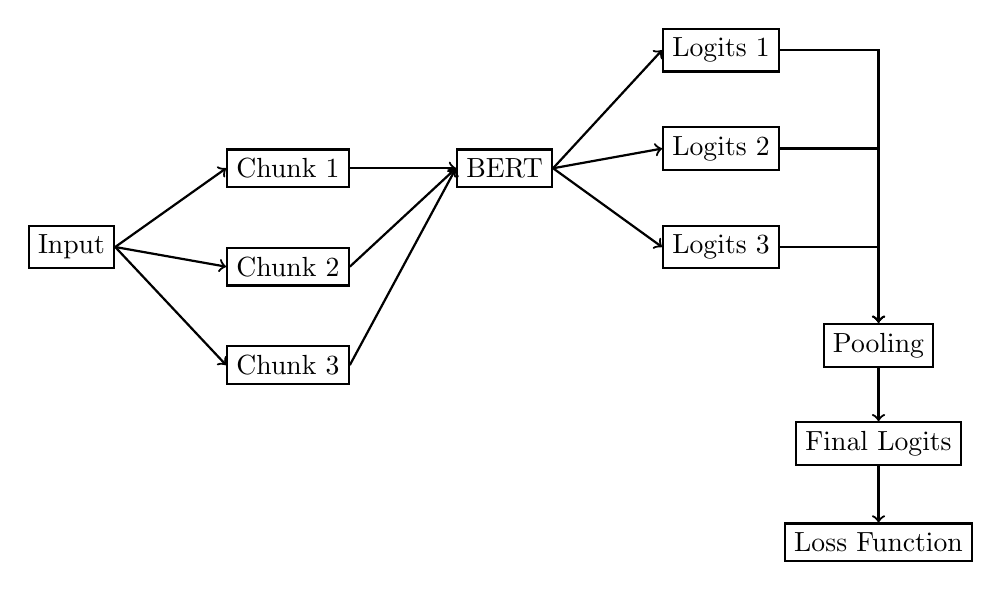
\begin{tikzpicture}[
            node distance=1.25cm,
            every node/.style={fill=white, font=\footnotesize},
            thick, scale=1, every node/.style={scale=1}
        ]

        \node (input) [draw, align=center] {Input};

        \node (chunk1) [draw, right of=input, xshift=1.5cm, yshift=1cm] {Chunk 1};
        \node (chunk2) [draw, below of=chunk1] {Chunk 2};
        \node (chunk3) [draw, below of=chunk2] {Chunk 3};

        \draw[->] (input.east) -- (chunk1.west);
        \draw[->] (input.east) -- (chunk2.west);
        \draw[->] (input.east) -- (chunk3.west);

        \node (bert) [draw, right of=chunk1, xshift=1.5cm] {BERT};

        \draw[->] (chunk1.east) -- (bert.west);
        \draw[->] (chunk2.east) -- (bert.west);
        \draw[->] (chunk3.east) -- (bert.west);

        \node (logits1) [draw, right of=bert, xshift=1.5cm, yshift=1.5cm] {Logits 1};
        \node (logits2) [draw, below of=logits1] {Logits 2};
        \node (logits3) [draw, below of=logits2] {Logits 3};

        \draw[->] (bert.east) -- (logits1.west);
        \draw[->] (bert.east) -- (logits2.west);
        \draw[->] (bert.east) -- (logits3.west);

        \node (pooling) [draw, below of=logits3, xshift=2cm, align=center] {Pooling};

        \draw[->] (logits1.east) -- ++(0.5cm,0) -| (pooling.north);
        \draw[->] (logits2.east) -- ++(0.5cm,0) -| (pooling.north);
        \draw[->] (logits3.east) -- ++(0.5cm,0) -| (pooling.north);

        \node (final_logits) [draw, below of=pooling] {Final Logits};

        \draw[->] (pooling.south) -- (final_logits.north);

        \node (loss) [draw, below of=final_logits] {Loss Function};

        \draw[->] (final_logits.south) -- (loss.north);
    \end{tikzpicture}
    \caption{Sliding window fine-tuning architecture. The input article is split into chunks, each chunk is processed by the model as a mini batch, and the resulting logits are pooled before applying the loss function.}
    \label{fig:sliding_window_architecture}
\end{figure}

Figure \ref{fig:sliding_window_architecture} illustrates the architecture of the sliding window method. Input texts are segmented into smaller chunks, which are then processed as mini-batches by the model. The logits (output scores) of each chunk are pooled together to produce final logits, to which the loss function is applied. This method bypasses the sequence length limitation of BERT models (512 tokens), allowing for full representation and processing of text input without any loss of information.

\begin{comment}
The complexity of this method is as follows:
\[
    O(L \cdot T \cdot H)
\]

where L is the sequence length, T is the number of transformer layers in the BERT model (typically 12), H is Hidden size of the BERT model (dimension of the transformer's feedforward networks, typically 768).
\end{comment}

\subsection{CLS method}


\begin{figure}[htbp]
    \centering

    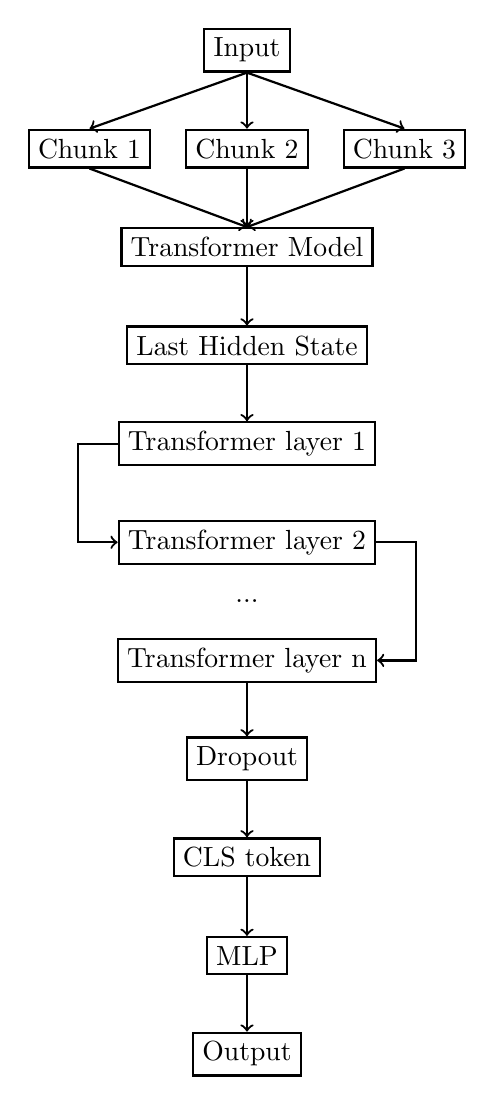
\begin{tikzpicture}[
            node distance=1.25cm,
            every node/.style={fill=white, font=\footnotesize},
            thick, scale=1, every node/.style={scale=1}]


        \node (input) [draw, align=center] {Input};

        \node (chunk1) [draw, below of=input, xshift=-2cm] {Chunk 1};
        \node (chunk2) [draw, below of=input] {Chunk 2};
        \node (chunk3) [draw, below of=input, xshift=2cm] {Chunk 3};

        \draw[->] (input.south) -- (chunk1.north);
        \draw[->] (input.south) -- (chunk2.north);
        \draw[->] (input.south) -- (chunk3.north);

        \node (encoder) [draw, below of=chunk2] {Transformer Model};

        \draw[->] (chunk1.south) -- (encoder.north);
        \draw[->] (chunk2.south) -- (encoder.north);
        \draw[->] (chunk3.south) -- (encoder.north);

        \node(hidden) [draw, below of=encoder] {Last Hidden State};

        \draw[->] (encoder.south) -- (hidden.north);

        \node (transformer1) [draw, below of=hidden] {Transformer layer 1};
        \node (transformer2) [draw, below of=transformer1] {Transformer layer 2};
        \node (transformern) [draw, below of=transformer2, yshift=-0.25cm] {Transformer layer n};
        \node (transformer_dots) [below of=transformer2, node distance=0.75cm] {...};

        \draw[->] (hidden.south) -- (transformer1.north);
        \draw[->] (transformer1.west) -- ++(-0.5cm,0) |- (transformer2.west);
        \draw[->] (transformer2.east) -- ++(0.5cm,0) |- (transformern.east);

        \node (dropout) [draw, below of=transformern] {Dropout};

        \draw[->] (transformern.south) -- (dropout.north);

        \node (cls) [draw, rectangle, below of=dropout] {CLS token};

        \draw[->] (dropout.south) -- (cls.north);

        \node (mlp) [draw, rectangle, below of=cls] {MLP};

        \draw[->] (cls.south) -- (mlp.north);

        \node (output) [draw, rectangle, below of=mlp] {Output};

        \draw[->] (mlp.south) -- (output.north);


    \end{tikzpicture}
    \caption{CLS method architecture}
    \label{fig:cls_method}
\end{figure}

Figure \ref{fig:cls_method} shows the full architecture of the CLS method.
This method begins by similarly segmenting the input text into smaller chunks. These chunks are encoded using a pre-trained Large Language Model (LLM) and fed into the model. The last hidden state, as described in \cite{sun-2020-fine-tune}, serves as the text representation. Subsequently, the chunks pass through multiple transformer layers to enrich their contextual understanding. For each chunk, only the representation of the CLS token (the first token) is retained (CLS Pooling, as in \cite{su-2021-classifying}), serving as a concise summary of the entire chunk sequence. This summary representation is then processed through a Multi-Layer Perceptron (MLP) layer. Finally, a softmax operation will be applied to the output of the MLP layer to determine the final output class.

Using a LLM as an encoder and taking its last hidden state allows for a good contextual representation of each chunk. By only using the CLS token representation instead of the whole chunk, this method allows for a more effective, yet simpler approach compared to other chunk pooling methods.

\begin{comment}
The complexity of the CLS method can be expressed as:
\[
    O(L \cdot TF \cdot T \cdot H_{\text{enc}}^2 \cdot M \cdot H_{\text{mlp}}^2)
\]

where:
\begin{align*}
    L              & : \text{Sequence length (number of tokens)}, \\
    T              & : \text{Number of transformer layers},       \\
    H_{\text{enc}} & : \text{Hidden size of transformer layers},  \\
    M              & : \text{Number of layers in the MLP},        \\
    H_{\text{mlp}} & : \text{Hidden size of the MLP}.             \\
\end{align*}
\end{comment}


%%% Local Variables: 
%%% mode: latex
%%% TeX-master: "thesis"
%%% End: 
